
{\underline {\bf В четвертой главе}} описано программный комплекс,
используемый для решения задачи определения инновационно-успешных предприятий.

Исходными данными задачи являются экономические данные по 135
наукоемким организациям в составе государственной корпорации «Ростех»:
внеоборотные активы (ВА), нематериальные активы (НМА), основные средства (ОС), оборотные
активы (ОА), запасы (ЗАП), дебиторская задолженность (ДЗ), собственный капитал (СК),
долгосрочные обязательства (ДО), краткосрочные обязательства (КО), кредиторская
задолженность (КЗ), выручка (В), себестоимость (С), материальные затраты (МЗ),
заработная плата (ЗП), амортизация (АМ), прочие затраты (ПЗ), коммерческие расходы (КР),
управленческие расходы (УР), прочие доходы (ПД), прочие расходы (ПР), расходы на
выплату процентов (РВП), прибыль до налогообложения (ПДН), налог на прибыль (НП),
чистая прибыль (ЧП), среднесписочная численность рабочих (ССЧР), среднегодовая
заработная плата (СГЗП), среднегодовые социальные выплаты (СГСВ).

Помимо экономических показателей известен кластер, содержащий инновационно-успешные
компании, определенный в работе к.т.н. Шиболденкова В. А.\footnote{
Шиболденков В. А. Разработка инструментария нейросетевого разведочного анализа и поддержки принятия решений по развитию экономических систем: Автореф. дис. канд. техн. наук. — Москва, 2019. — 24 с.
}

Постновка задачи, решаемой в диссертационном исследовании, звучит следующим образом:
необходимо принять решение, какие $N$ компаний следует инвестировать с минимальным риском.
Данная задача может быть решена с помощью РС сведением ее к задаче $topN$.
Объектами РС являются предприятия, экономические показатели --- характеристики, значение
показателя --- значение характеристики. Поиск $N$ объектов, удовлетворяющих некоторому критерию --- это задача $topN$.
Для сведения постановки задачи к задаче $topN$ необходимо сформировать контент активного пользователя.

Для решения задачи применялась НКМ. Решение задачи $topN$ заключается в поиске объектов, между которыми и активным пользователем
расстояние минимально. Поэтому было принято решение формировать контент активного из данных экономических показателей, которые
являются факторами, влияющими на кластеризацию предприятий. Существование кластера подтверждается работой Шиболденкова В. А. 

Определение факторных характеристик и построение контента активного пользователя производится по следующему алгоритмы:
\begin{enumerate}
\item из множества всех объектов, формируется кластер объектов, между которыми выполняется свойство отношения близости;
\item производится выборка таких характеристик объектов, определенных на шаге 1, между которыми существует корелляция;
\item контент активного пользователя состоит из характеристик, определенных на шаге 2, значениями которых является среднее значение.
\end{enumerate}

Программный комплекс состоит из следующих компонент:
\begin{itemize}
	\item BRAVO --- база знаний. Применяется для хранения данных о предприятиях;
	\item Rand Model Designer --- система иммитационного моделирования бизнес процессов. Применяется для решения задачи $topN$
		по данным, хранящимся в базе знаний и результатам проведенного кластерного анализа для выявления факторных характеристик;
	\item скрипт, написанный на языке Python, который производит кластерный анализ для выявления факторных характестик и интеграцию
		данных BRAVO и Rand Model Designer.
\end{itemize}

\begin{figure}[H]
	\caption{UML-диаграмма программного комплекса}
	\begin{center}
		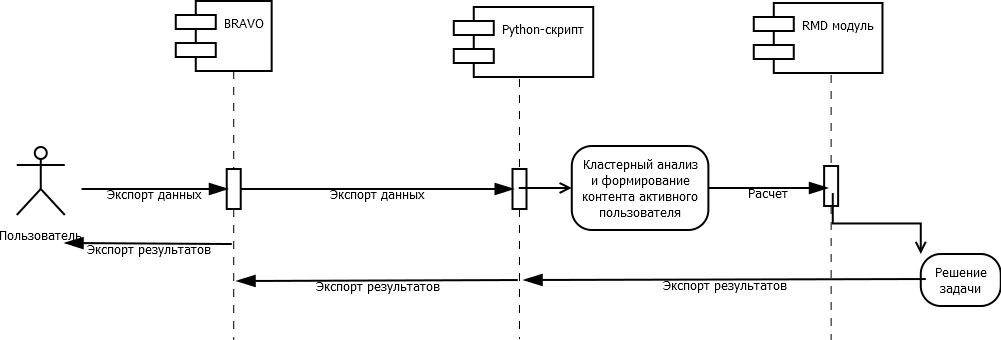
\includegraphics[width=6in,height=3in]{pics/integration.png}
	\end{center}
\end{figure}

Для выявления показателя качества решения было проведено тестирование, состоящее из следующих итераций:
\begin{enumerate}
	\item исходное множество данных, состоящее из 135 предприятий случайным разбивается на обчающее и тестовое множество в соотношение 4 к 1 соответсвенно;
	\item по обучающему множество проводится кластерный анализ для определения факторных характеристик и формирования контента активного пользователя;
	\item производится решение задачи $topN$;
	\item вычисляется показатель качества решения: $\frac{N'}{N}$, где $N'$ --- число объектов решения, которые входят в кластер инновационно-успешных предприятий,
		$M$ --- мощность кластера;
\end{enumerate}
Цикл тестовых операций был проведен порядка 1000 раз. Средний показатель качества равен 0,9. То есть определение инновационно-успешных предприятий производится с точностью
90\% при применении НКМ.


{\underline {\bf В приложении}} проведено тестирование АКМ и НКМ на множестве данных MovieLens
при решении задач $topN$ и $pred$.
Характеристики используемого множества данных:
\begin{itemize}
	\item $|U| = 700$;
	\item $|I| = 9000$ --- объектами являются фильмы
	\item $|P| = 100 000$ --- значениями $\rho(u, i)$ являются оценки
		пользователей, которые были ими заданы в соответствии со своим
		предпочтением к конкретному фильму;
	\item $|Y|$ --- характеристиками объектов являются кинематографические
		жанры;
	\item $X = I$ --- характеристиками пользователей для АКМ являются объекты.
\end{itemize}

Для АКМ $X = I$ и $w_U(u, x) = \rho(u,x), x \in I$.

Для задания правила вывода $\Pi_f$ была аналитически определена
функция $\delta_c$, основываясь на эвристическом предположении о том,
что между оценкой близости $\rho(u, i)$, заданной пользователем $u$
и характеристикой $y \in Y$ объекта $i$,
то есть жанром фильма, существует корреляция:
\begin{multline}
	\delta_c(i, y) = \frac{1}{|\{i: \exists \rho(u,i)\}|}
	\cdot
	|\{ i : (\rho(u, i) < \varepsilon_1) \wedge (\nu(y) = 1)\}| -\\
	|\{ i : (\rho(u, i) > \varepsilon_2) \wedge (\nu(y) = 1)\}|, \\
	\text{ где }
	\varepsilon_1 = 0,2, \varepsilon_2 = 0,6;
\end{multline}

Такое эвристическое предположение верно не для всех пользователей, так как
их вкусы могут быть неоднородными. Поэтому для некоторых пользователей функция
$\delta_c$ задана так, что
$|\rh(u, i_{\bot}) - \rho(u, i_{\bot}) \le \varepsilon_p|$,
а для некоторых --- нет.

В таблицах приведены значения оценок качества (точность для задачи $topN$ и NMAE для задачи $pred$).
Полученные результаты подтверждают теоретический вывод о том, что НКМ является качественным расширением АКМ.

\begin{table}[htb]
	\caption{Задача $p$}
  \begin{center}
	\label{table:p}
	\begin{tabular}{|c|c|}
	  \hline
		Модель/Правило вычисления & NAME \\ \hline
		АКМ/$\Pi_{COM}$&0,23 \\ \hline
		НКМ/$\Pi_{COM}$&0,13 \\ \hline
		НКМ/$\Pi_{f}$&0,11 \\ \hline
	\end{tabular}
  \end{center}
\end{table}

\begin{table}[htb]
	\caption{Задача $topN$}
  \begin{center}
	\label{table:topn}
	\begin{tabular}{|c|c|}
	  \hline
		Модель/Правило вычисления & Точность \\ \hline
		АКМ/$\Pi_{OOM}$&0,32 \\ \hline
		НКМ/$\Pi_{OOM}$&0,53 \\ \hline
		НКМ/$\Pi_{f}$&0,81 \\ \hline
	\end{tabular}
  \end{center}
\end{table}

